\begin{FPfigure}

\begin{center}
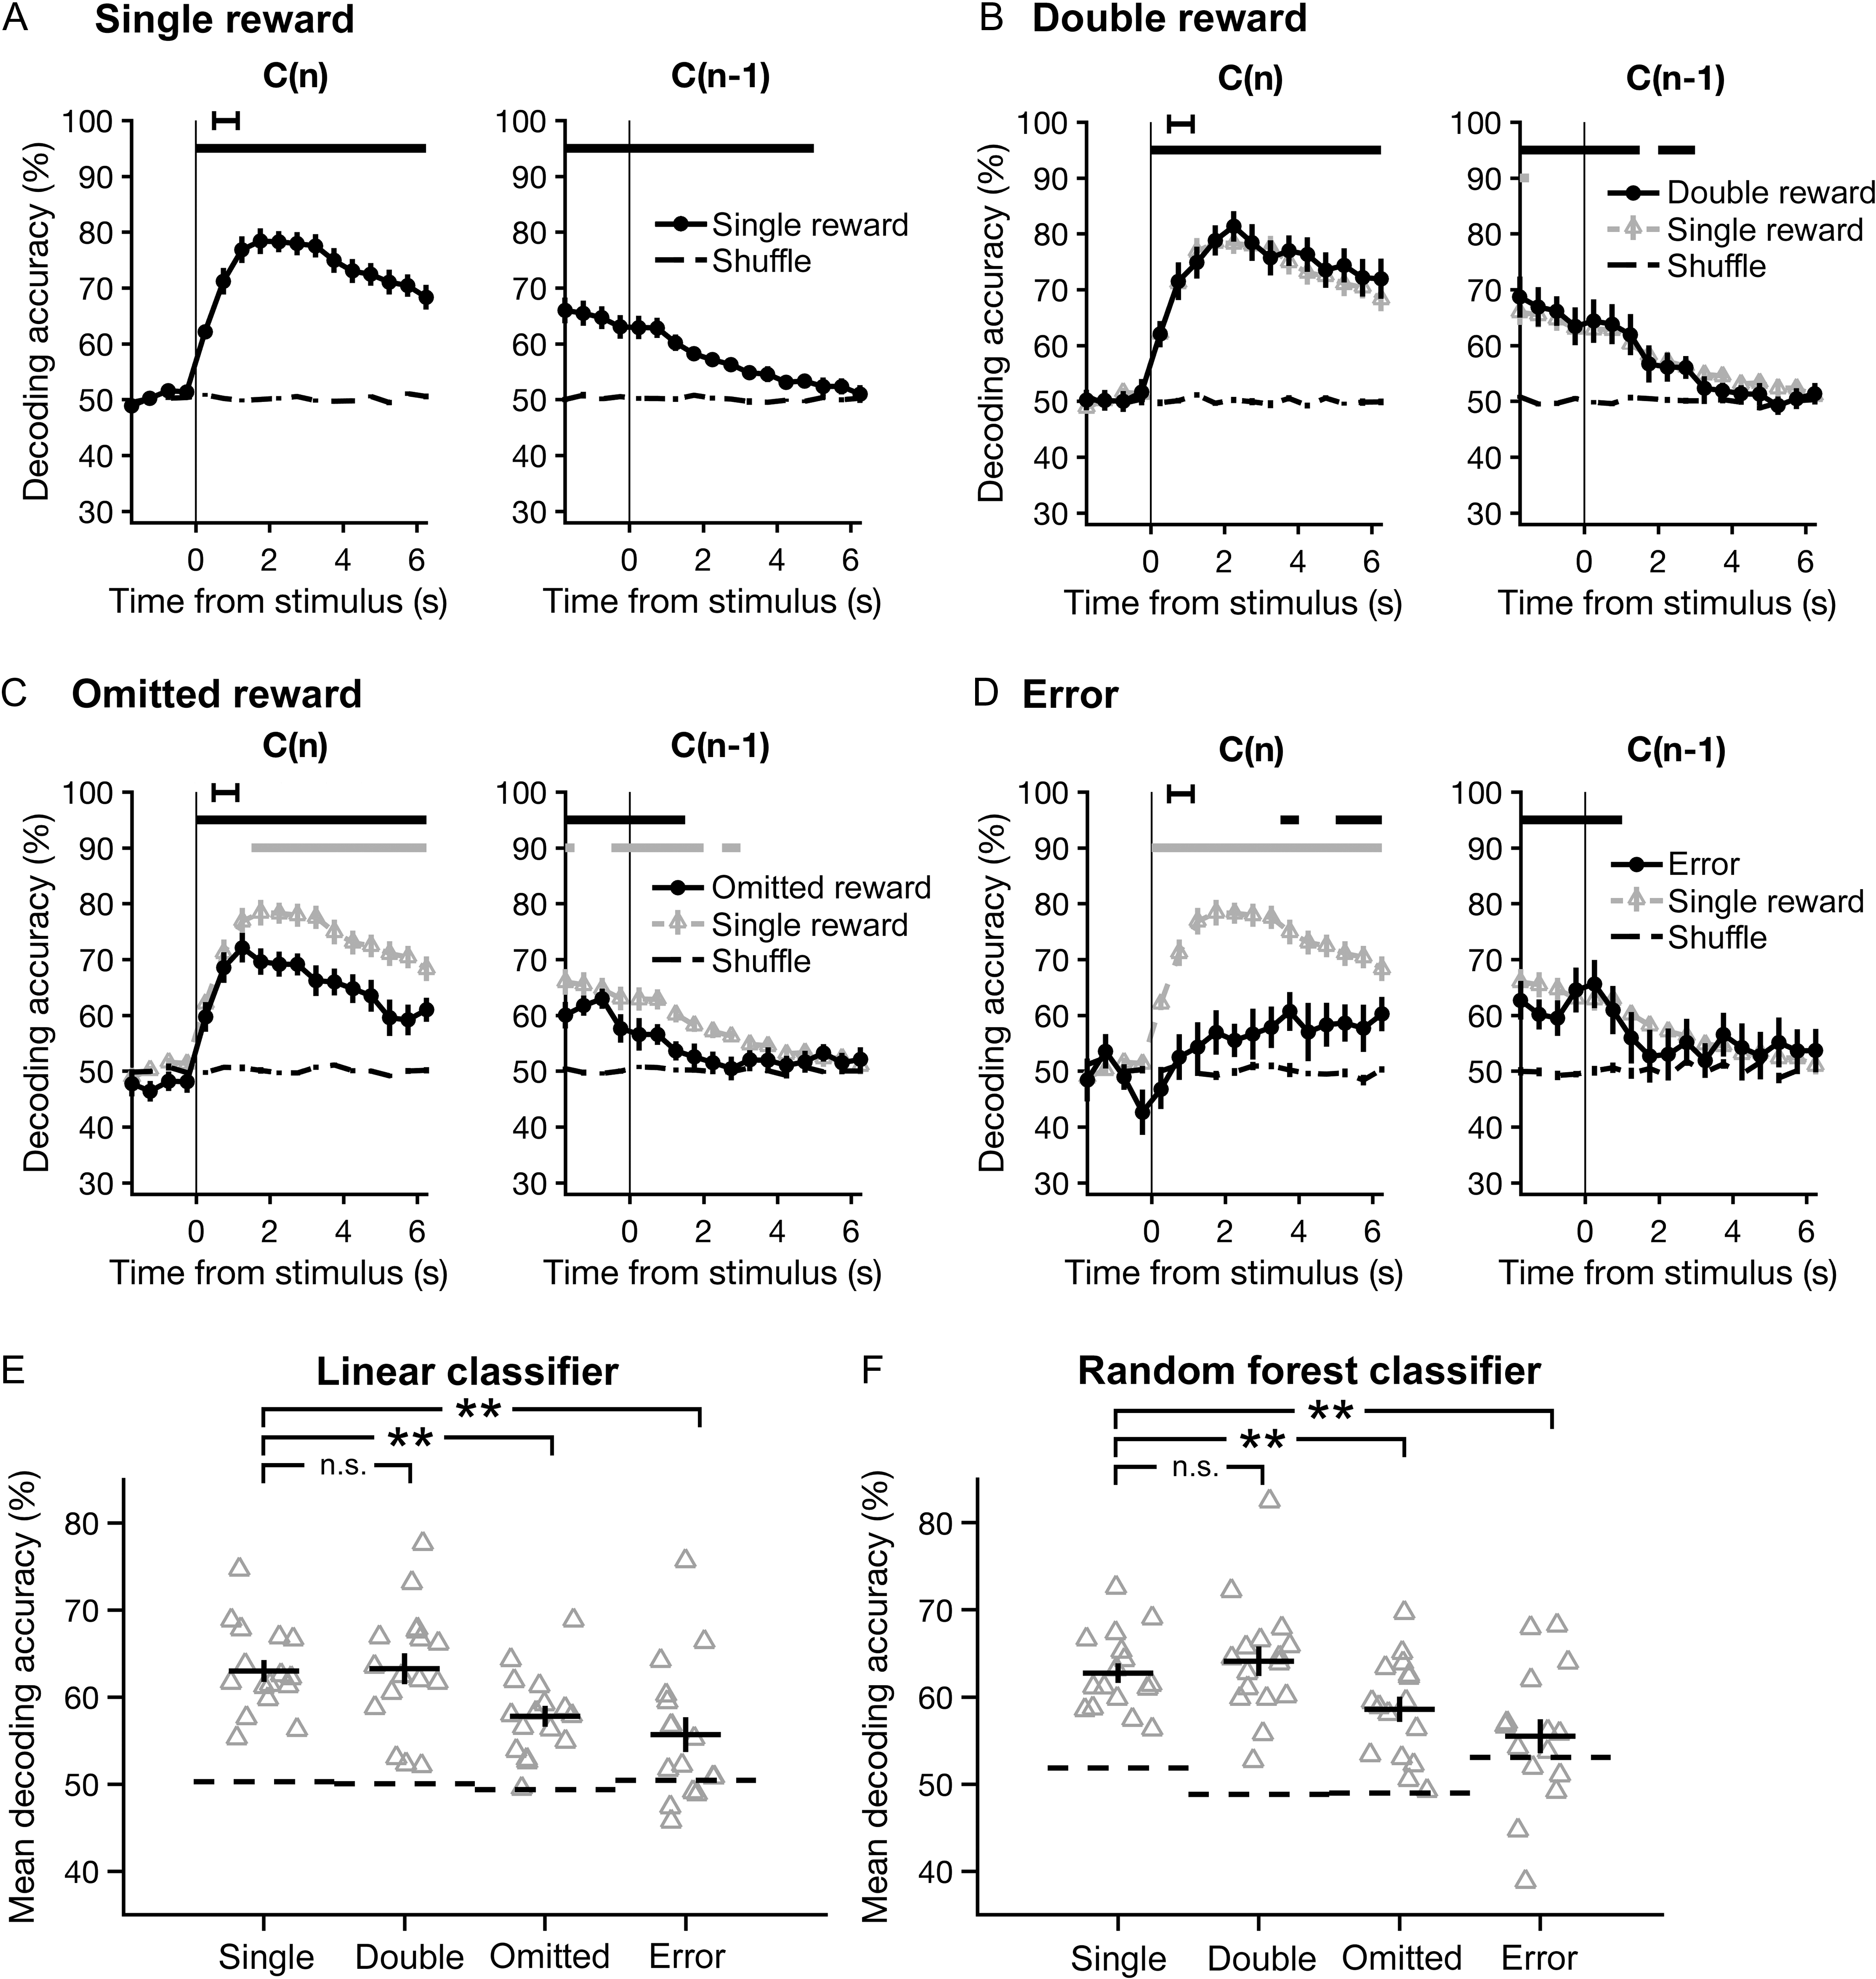
\includegraphics[width=\textwidth]{Figures/Chapter2/CC_fig6} 
\small{Figure \ref{fig:CC_fig6}: Decoding accuracy diminished during omitted-reward and error trials. }
\end{center}

\caption[Decoding accuracy diminished during omitted-reward and error trials]
{The accuracy of decoding chosen actions from the neural ensemble activity was diminished during omitted-reward and error trials. Choices were decoded using classifiers based on linear discriminant analysis, and accuracy was estimated with Monte Carlo cross-validation (repeated random subsampling). (A) The accuracy of decoding choices made on single-reward trials (left), or trials in which the previous outcome was single reward (right), plotted as a function of time. Data are presented as $\mathit{mean}\pm\mathit{SEM}$. Chance-level accuracy (black dashed line) was determined by testing classifiers constructed using shuffled choices. Black horizontal bars, bins significantly different from chance ($p < 0.05$, Wilcoxon signed-rank test). Black error bar, 95\% confidence interval for time of outcome. (B-D) Same as A for double-reward, omitted-reward, and error trials. Results from single-reward trials are overlaid for visual comparison (gray triangles). Lower gray bars, bins with a significant difference in decoding accuracy relative to single-reward trials. (E) Mean decoding accuracy across all time-points shown in A–D for each trial outcome. Gray triangles, individual sessions. Black crosshairs, $\mathit{mean}\pm\mathit{SEM}$. Wilcoxon signed-rank test: **$p < 0.01$; n.s., not significant. (F) Same as E using random forest classifiers.}
% \clearpage %\placefloats places without an automatic new page
\label{fig:CC_fig6}
\end{FPfigure}